\documentclass[11pt]{article}\usepackage[]{graphicx}\usepackage[]{color}
% maxwidth is the original width if it is less than linewidth
% otherwise use linewidth (to make sure the graphics do not exceed the margin)
\makeatletter
\def\maxwidth{ %
  \ifdim\Gin@nat@width>\linewidth
    \linewidth
  \else
    \Gin@nat@width
  \fi
}
\makeatother

\definecolor{fgcolor}{rgb}{0.345, 0.345, 0.345}
\newcommand{\hlnum}[1]{\textcolor[rgb]{0.686,0.059,0.569}{#1}}%
\newcommand{\hlstr}[1]{\textcolor[rgb]{0.192,0.494,0.8}{#1}}%
\newcommand{\hlcom}[1]{\textcolor[rgb]{0.678,0.584,0.686}{\textit{#1}}}%
\newcommand{\hlopt}[1]{\textcolor[rgb]{0,0,0}{#1}}%
\newcommand{\hlstd}[1]{\textcolor[rgb]{0.345,0.345,0.345}{#1}}%
\newcommand{\hlkwa}[1]{\textcolor[rgb]{0.161,0.373,0.58}{\textbf{#1}}}%
\newcommand{\hlkwb}[1]{\textcolor[rgb]{0.69,0.353,0.396}{#1}}%
\newcommand{\hlkwc}[1]{\textcolor[rgb]{0.333,0.667,0.333}{#1}}%
\newcommand{\hlkwd}[1]{\textcolor[rgb]{0.737,0.353,0.396}{\textbf{#1}}}%
\let\hlipl\hlkwb

\usepackage{framed}
\makeatletter
\newenvironment{kframe}{%
 \def\at@end@of@kframe{}%
 \ifinner\ifhmode%
  \def\at@end@of@kframe{\end{minipage}}%
  \begin{minipage}{\columnwidth}%
 \fi\fi%
 \def\FrameCommand##1{\hskip\@totalleftmargin \hskip-\fboxsep
 \colorbox{shadecolor}{##1}\hskip-\fboxsep
     % There is no \\@totalrightmargin, so:
     \hskip-\linewidth \hskip-\@totalleftmargin \hskip\columnwidth}%
 \MakeFramed {\advance\hsize-\width
   \@totalleftmargin\z@ \linewidth\hsize
   \@setminipage}}%
 {\par\unskip\endMakeFramed%
 \at@end@of@kframe}
\makeatother

\definecolor{shadecolor}{rgb}{.97, .97, .97}
\definecolor{messagecolor}{rgb}{0, 0, 0}
\definecolor{warningcolor}{rgb}{1, 0, 1}
\definecolor{errorcolor}{rgb}{1, 0, 0}
\newenvironment{knitrout}{}{} % an empty environment to be redefined in TeX

\usepackage{alltt}

\usepackage[T1]{fontenc}
\usepackage[polish]{babel}
\usepackage[utf8]{inputenc}
\usepackage{lmodern}
\selectlanguage{polish}
\usepackage{graphicx}
\usepackage{float}
\usepackage[a4paper, total={6.5in, 8.5in}]{geometry}
\usepackage{amsmath}
\usepackage{amsfonts}
\usepackage[hidelinks]{hyperref}
\usepackage{tabularx}

\urlstyle{rm}
  
\usepackage{setspace}
\newtheorem{stat}{Statement}
\newtheorem{theorem}{Theorem}
\newtheorem{defi}{Definition}
\newtheorem{lem}[stat]{Lemma}
\newtheorem{ex}{Example}[section]
\newtheorem{fact}{Fact}

\frenchspacing
\IfFileExists{upquote.sty}{\usepackage{upquote}}{}
\begin{document}


\title{Bank Marketing data (with social/economic context)}
\author{Maciej Ma戼㸳ecki}
\maketitle
\abstract{W pliku Bank Marketing data.csv znajduj戼㸹 si攼㹡 dane charakteryzuj戼㸹ce klient昼㸳w pewnego banku oraz kampanie marketingowe skierowane do tych klient昼㸳w. Do戼㸳戼㸹czone s戼㸹 ponadto wska㤼㹦niki spo戼㸳eczne i ekonomiczne. Na podstawie tych danych nale戼㹦y zbudowa攼㸶 model prognozuj戼㸹cy szans攼㹡, 戼㹦e klient w wyniku prowadzonej kampanii za戼㸳o戼㹦y lokat攼㹡 terminow戼㸹.}
\tableofcontents

\newpage

\section{Wprowadzenie}
\subsection{Opis problemu}
W ramach kampani marketingowej organizowanej przez pewien bank w latach mi攼㹡dzy majem 2008 rok, a listopadem 2010 roku, by戼㸳y zbierane informacje na temat klient昼㸳w tego banku. 
Na podstawie tych danych planowane jest przewidzenie, czy i jakie rodzaj klient昼㸳w kupi lokat攼㹡 terminow戼㸹 w tym banku.

\subsection{Opis danych}
Nasze dane zawieraj戼㸹 21 column danych. Kolumny mo戼㹦emy podzieli攼㸶 na 3 grupy:

\textbf{I: Zmienne zwi戼㸹zane z danymi klienta bankowego:}

\begin{enumerate}
\item Wiek (age): wiek klienta.
\item Praca (job): rodzaj pracy klienta.
\item Stan cywilny (marital): stan cywilny klienta.
\item Edukacja (education): edukacja klienta.
\item Domy㤼㹣lnie (default): Klient wcze㤼㹣niej domy㤼㹣lnie mia戼㸳 kredyt.
\item Mieszkanie (housing): Klient ma kredyt mieszkaniowy.
\item Po戼㹦yczka (loan): Klient ma osobist戼㸹 po戼㹦yczk攼㹡.
\end{enumerate}


\textbf{II: Zmienne zwi戼㸹zane z ostatnim kontaktem bie戼㹦戼㸹cej kampanii marketingowej:}

\begin{enumerate}
\setcounter{enumi}{7}
\item Kontakt (contact): Typ komunikacji kontaktowej (telefonicznej lub kom昼㸳rkowej).
\item Miesi戼㸹c (month): Ostatni kontakt miesi戼㸹ca roku.
\item Dzie昼㸱 tygodnia (day of week): dzie昼㸱 ostatniego kontaktu tygodnia.
\item Czas trwania (duration): czas trwania ostatniego kontaktu w sekundach. Je㤼㹣li czas trwania wynosi 0, nigdy nie skontaktowali㤼㹣my si攼㹡 z klientem, aby za戼㸳o戼㹦y攼㸶 konto lokaty terminowej.
\item Kampania (campaign): liczba kontakt昼㸳w wykonanych podczas tej kampanii i dla tego klienta
\item Liczba dni (pdays): liczba dni, kt昼㸳re up戼㸳yn攼㹡戼㸳y od ostatniego kontaktu klienta z poprzedniej kampanii (warto㤼㹣攼㸶 liczbowa; 999 oznacza, 戼㹦e klient wcze㤼㹣niej si攼㹡 nie skontaktowa戼㸳)
\item Poprzedni (previous): liczba kontakt昼㸳w wykonanych przed t戼㸹 kampani戼㸹 i dla tego klienta (numerycznie)
\item Poutcome: wynik poprzedniej kampanii marketingowej (kategorycznie: 㠼㸴pora戼㹦ka㤼㸴, 㠼㸴nieistniej戼㸹ca㤼㸴, 㠼㸴sukces㤼㸴)
\end{enumerate}

\textbf{III: Atrybuty kontekstu spo戼㸳ecznego i gospodarczego:}

\begin{enumerate}
\setcounter{enumi}{15}
\item Emp.var.rate: wska㤼㹦nik zmienno㤼㹣ci zatrudnienia - wska㤼㹦nik kwartalny 
\item Cons.price.idx: wska㤼㹦nik cen konsumpcyjnych - wska㤼㹦nik miesi攼㹡czny 
\item Cons.conf.idx: wska㤼㹦nik zaufania konsument昼㸳w - wska㤼㹦nik miesi攼㹡czny 
\item Euribor3m: stawka 3-miesi攼㹡czna euribor - wska㤼㹦nik dzienny 
\item Liczba zatrudnionych (nr employed): liczba pracownik昼㸳w - wska㤼㹦nik kwartalny 
\end{enumerate}


\textbf{Zmienna wyj㤼㹣ciowa (po戼㹦戼㸹dany cel):}

\begin{enumerate}
\setcounter{enumi}{20}
\item y - czy klient subskrybowa戼㸳 lokat攼㹡? (dw昼㸳jkowy: 㠼㸴tak㤼㸴, 㠼㸴nie㤼㸴)
\end{enumerate}

\subsection{Wst攼㹡pna eksploracja danych}
\begin{knitrout}
\definecolor{shadecolor}{rgb}{0.969, 0.969, 0.969}\color{fgcolor}\begin{kframe}


{\ttfamily\noindent\bfseries\color{errorcolor}{\#\# Error in contrib.url(repos, "{}source"{}): trying to use CRAN without setting a mirror}}

{\ttfamily\noindent\bfseries\color{errorcolor}{\#\# Error in contrib.url(repos, "{}source"{}): trying to use CRAN without setting a mirror}}

{\ttfamily\noindent\bfseries\color{errorcolor}{\#\# Error in contrib.url(repos, "{}source"{}): trying to use CRAN without setting a mirror}}

{\ttfamily\noindent\bfseries\color{errorcolor}{\#\# Error in contrib.url(repos, "{}source"{}): trying to use CRAN without setting a mirror}}

{\ttfamily\noindent\bfseries\color{errorcolor}{\#\# Error in contrib.url(repos, "{}source"{}): trying to use CRAN without setting a mirror}}

{\ttfamily\noindent\bfseries\color{errorcolor}{\#\# Error in contrib.url(repos, "{}source"{}): trying to use CRAN without setting a mirror}}

{\ttfamily\noindent\bfseries\color{errorcolor}{\#\# Error in contrib.url(repos, "{}source"{}): trying to use CRAN without setting a mirror}}

{\ttfamily\noindent\bfseries\color{errorcolor}{\#\# Error in contrib.url(repos, "{}source"{}): trying to use CRAN without setting a mirror}}

{\ttfamily\noindent\bfseries\color{errorcolor}{\#\# Error in contrib.url(repos, "{}source"{}): trying to use CRAN without setting a mirror}}

{\ttfamily\noindent\bfseries\color{errorcolor}{\#\# Error in contrib.url(repos, "{}source"{}): trying to use CRAN without setting a mirror}}

{\ttfamily\noindent\bfseries\color{errorcolor}{\#\# Error in contrib.url(repos, "{}source"{}): trying to use CRAN without setting a mirror}}

{\ttfamily\noindent\bfseries\color{errorcolor}{\#\# Error in contrib.url(repos, "{}source"{}): trying to use CRAN without setting a mirror}}\end{kframe}
\end{knitrout}


Badane dane zawieraj� 4119 wierszy oraz 21 kolumn o nast�puj�cych nazwach:

\begin{knitrout}
\definecolor{shadecolor}{rgb}{0.969, 0.969, 0.969}\color{fgcolor}\begin{kframe}
\begin{verbatim}
##  [1] "age"            "job"            "marital"        "education"     
##  [5] "default"        "housing"        "loan"           "contact"       
##  [9] "month"          "day_of_week"    "duration"       "campaign"      
## [13] "pdays"          "previous"       "poutcome"       "emp.var.rate"  
## [17] "cons.price.idx" "cons.conf.idx"  "euribor3m"      "nr.employed"   
## [21] "y"
\end{verbatim}
\end{kframe}
\end{knitrout}

Struktura danych:
\begin{knitrout}
\definecolor{shadecolor}{rgb}{0.969, 0.969, 0.969}\color{fgcolor}\begin{kframe}
\begin{alltt}
\hlkwd{str}\hlstd{(df_bank)}
\end{alltt}
\begin{verbatim}
## 'data.frame':	4119 obs. of  21 variables:
##  $ age           : int  30 39 25 38 47 32 32 41 31 35 ...
##  $ job           : chr  "blue-collar" "services" "services" "services" ...
##  $ marital       : chr  "married" "single" "married" "married" ...
##  $ education     : chr  "basic.9y" "high.school" "high.school" "basic.9y" ...
##  $ default       : chr  "no" "no" "no" "no" ...
##  $ housing       : chr  "yes" "no" "yes" "unknown" ...
##  $ loan          : chr  "no" "no" "no" "unknown" ...
##  $ contact       : chr  "cellular" "telephone" "telephone" "telephone" ...
##  $ month         : chr  "may" "may" "jun" "jun" ...
##  $ day_of_week   : chr  "fri" "fri" "wed" "fri" ...
##  $ duration      : int  487 346 227 17 58 128 290 44 68 170 ...
##  $ campaign      : int  2 4 1 3 1 3 4 2 1 1 ...
##  $ pdays         : int  999 999 999 999 999 999 999 999 999 999 ...
##  $ previous      : int  0 0 0 0 0 2 0 0 1 0 ...
##  $ poutcome      : chr  "nonexistent" "nonexistent" "nonexistent" "nonexistent" ...
##  $ emp.var.rate  : num  -1.8 1.1 1.4 1.4 -0.1 -1.1 -1.1 -0.1 -0.1 1.1 ...
##  $ cons.price.idx: num  92.9 94 94.5 94.5 93.2 ...
##  $ cons.conf.idx : num  -46.2 -36.4 -41.8 -41.8 -42 -37.5 -37.5 -42 -42 -36.4 ...
##  $ euribor3m     : num  1.31 4.86 4.96 4.96 4.19 ...
##  $ nr.employed   : num  5099 5191 5228 5228 5196 ...
##  $ y             : chr  "no" "no" "no" "no" ...
\end{verbatim}
\end{kframe}
\end{knitrout}

Czy w danych znajduj� si� warto�ci typu \verb+NaN+ lub \verb+Na+ ?
\begin{knitrout}
\definecolor{shadecolor}{rgb}{0.969, 0.969, 0.969}\color{fgcolor}\begin{kframe}
\begin{verbatim}
## [1] FALSE
\end{verbatim}
\end{kframe}
\end{knitrout}

Jednak�e wiemy, �e w danych wyst�puj� warto�ci brakuj�ce i s� one opisa "unknown". W danych znajduje si� 1230  rekord�w z warto�ci� "unknown" rozmieszczonych w 1029 r�nych wierszach. To stanowi $24.98\% $ wszystkich wierszy w naszej badzie danych, wi�c nie mo�emy pozwoli� sobie na usuni�cie tych wszystkich informacji. W tabeli 1 znajduj� si� informacje na temat liczny nieznanych warto�ci  w ka�dej z kolumn z osobna.




\begin{knitrout}
\definecolor{shadecolor}{rgb}{0.969, 0.969, 0.969}\color{fgcolor}\begin{kframe}


{\ttfamily\noindent\bfseries\color{errorcolor}{\#\# Error: nie znaleziono obiektu 'Number\_of\_unknown'}}

{\ttfamily\noindent\bfseries\color{errorcolor}{\#\# Error in kable(table\_unknown, "{}latex"{}, booktabs = F, caption = "{}Liczba nieznanych warto<U+009C>ci w poszczegulnych kolumnach."{}): nie znaleziono obiektu 'table\_unknown'}}\end{kframe}
\end{knitrout}


\section{Analiza eksploracyjna}


W tej sekcji zostanie om�wiony ka�dy parametr z osobna. Nast�pnie dane zostan� odpowiednio przygotowane do wykorzystania ich w modelach predykcyjnych.

\subsection{Age}
W jakim wieku by�y osoby, z kt�rymi skontaktowano si� podczas tej kampani?



\begin{knitrout}
\definecolor{shadecolor}{rgb}{0.969, 0.969, 0.969}\color{fgcolor}\begin{kframe}


{\ttfamily\noindent\bfseries\color{errorcolor}{\#\# Error in dimnames(x) <- dnx: 'dimnames()' zastosowane do nie-tablicy}}\end{kframe}
\end{knitrout}

\begin{knitrout}
\definecolor{shadecolor}{rgb}{0.969, 0.969, 0.969}\color{fgcolor}\begin{figure}[H]

{\centering 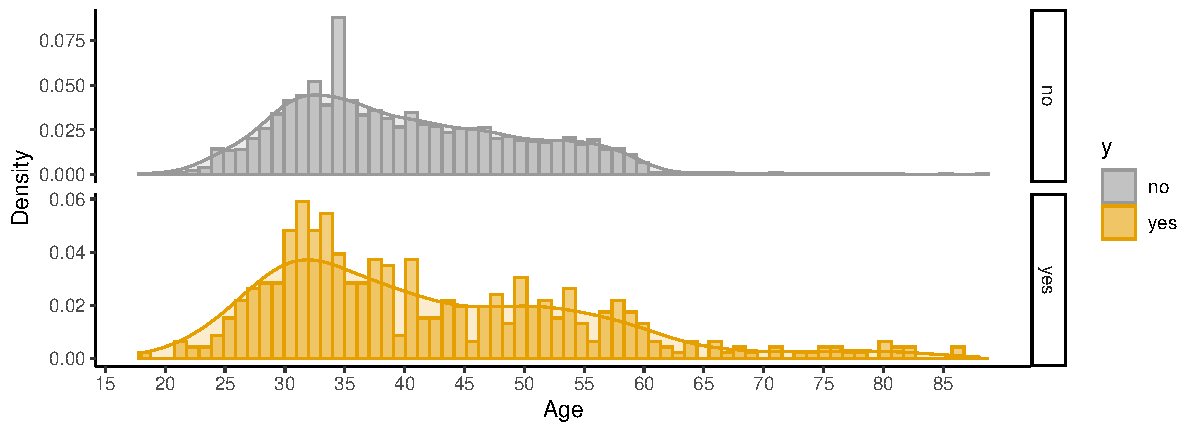
\includegraphics[width=\maxwidth]{figure/unnamed-chunk-10-1} 

}

\caption[Histogram wieku klient<U+663C><U+3E33>w w zale<U+623C><U+3E66>no<U+393C><U+3E63>ci od wzi<U+653C><U+3E61>cia lokaty d<U+623C><U+3E33>ugoterminowej]{Histogram wieku klient<U+663C><U+3E33>w w zale<U+623C><U+3E66>no<U+393C><U+3E63>ci od wzi<U+653C><U+3E61>cia lokaty d<U+623C><U+3E33>ugoterminowej.}\label{fig:unnamed-chunk-10}
\end{figure}


\end{knitrout}

\begin{knitrout}
\definecolor{shadecolor}{rgb}{0.969, 0.969, 0.969}\color{fgcolor}\begin{figure}[H]

{\centering 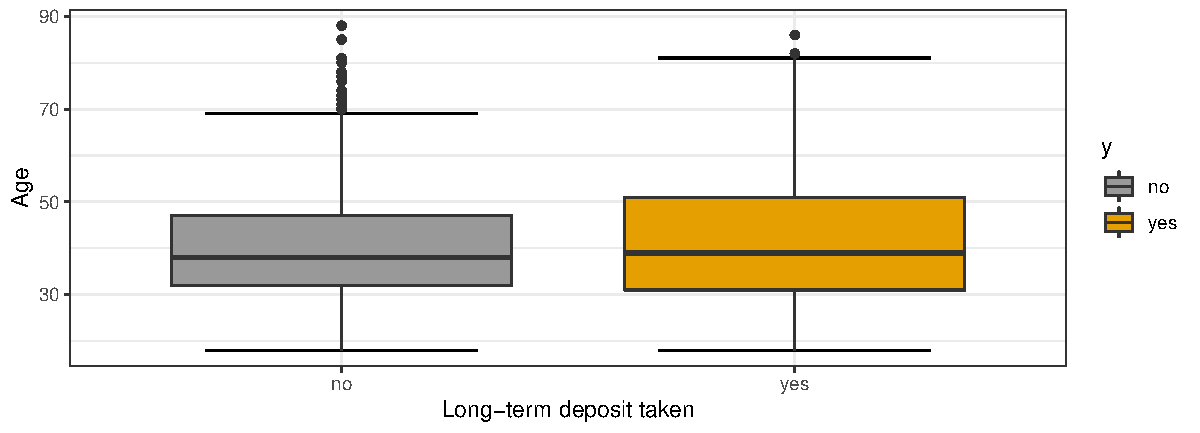
\includegraphics[width=\maxwidth]{figure/unnamed-chunk-11-1} 

}

\caption[Boxplot wieku klient<U+663C><U+3E33>w w zale<U+623C><U+3E66>no<U+393C><U+3E63>ci od wzi<U+653C><U+3E61>cia lokaty d<U+623C><U+3E33>ugoterminowej]{Boxplot wieku klient<U+663C><U+3E33>w w zale<U+623C><U+3E66>no<U+393C><U+3E63>ci od wzi<U+653C><U+3E61>cia lokaty d<U+623C><U+3E33>ugoterminowej.}\label{fig:unnamed-chunk-11}
\end{figure}


\end{knitrout}






\subsection{}



\begin{knitrout}
\definecolor{shadecolor}{rgb}{0.969, 0.969, 0.969}\color{fgcolor}\begin{figure}[H]

{\centering 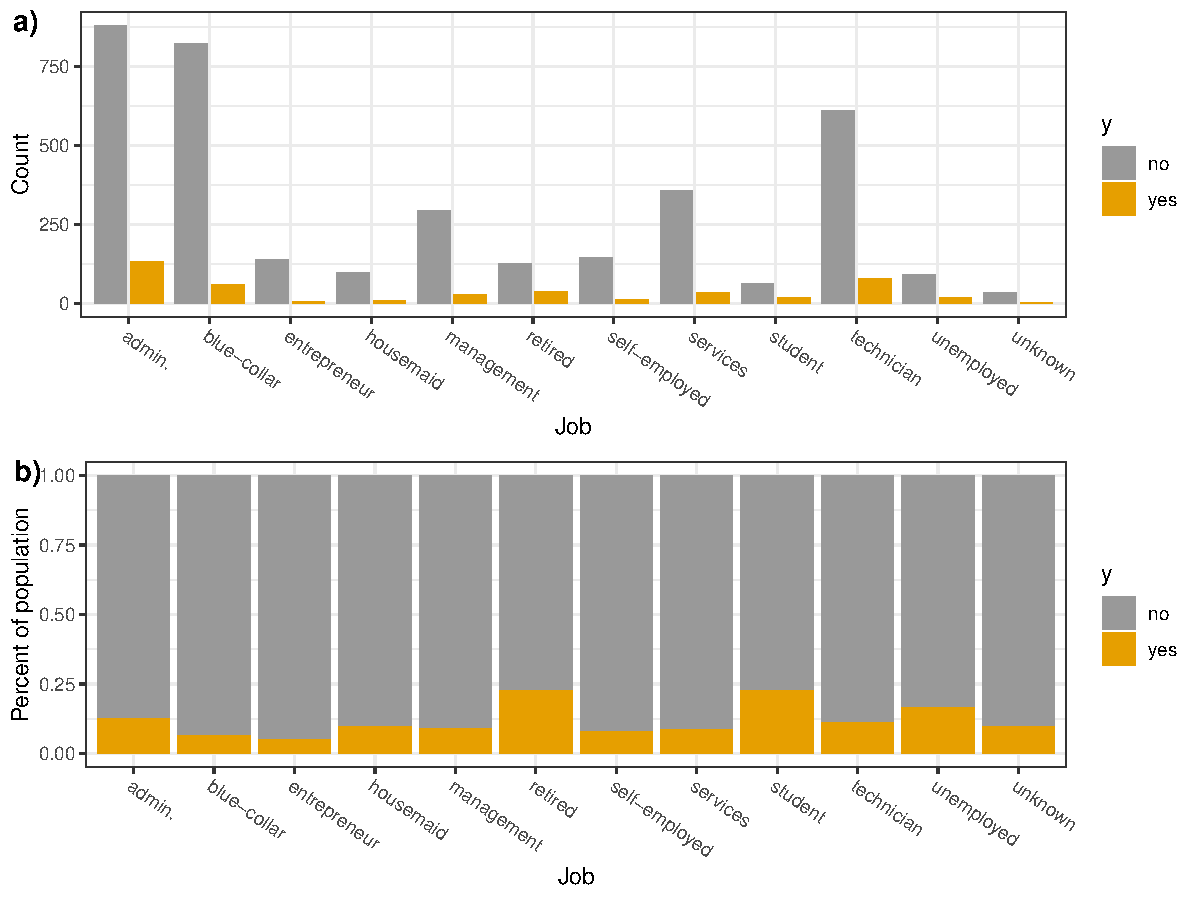
\includegraphics[width=\maxwidth]{figure/unnamed-chunk-13-1} 

}

\caption[New Figure]{New Figure}\label{fig:unnamed-chunk-13}
\end{figure}


\end{knitrout}

\begin{knitrout}
\definecolor{shadecolor}{rgb}{0.969, 0.969, 0.969}\color{fgcolor}\begin{figure}[H]

{\centering 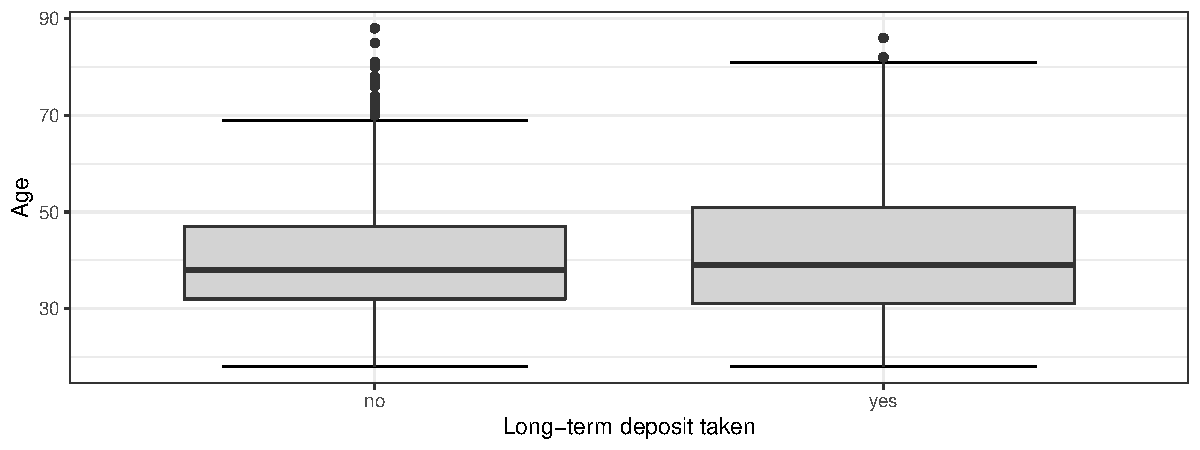
\includegraphics[width=\maxwidth]{figure/unnamed-chunk-14-1} 

}

\caption[New Figure]{New Figure}\label{fig:unnamed-chunk-14}
\end{figure}


\end{knitrout}

\begin{knitrout}
\definecolor{shadecolor}{rgb}{0.969, 0.969, 0.969}\color{fgcolor}\begin{kframe}


{\ttfamily\noindent\bfseries\color{errorcolor}{\#\# Error in dimnames(x) <- dnx: 'dimnames()' zastosowane do nie-tablicy}}\end{kframe}
\end{knitrout}


\subsection{}



\begin{knitrout}
\definecolor{shadecolor}{rgb}{0.969, 0.969, 0.969}\color{fgcolor}\begin{figure}[H]

{\centering 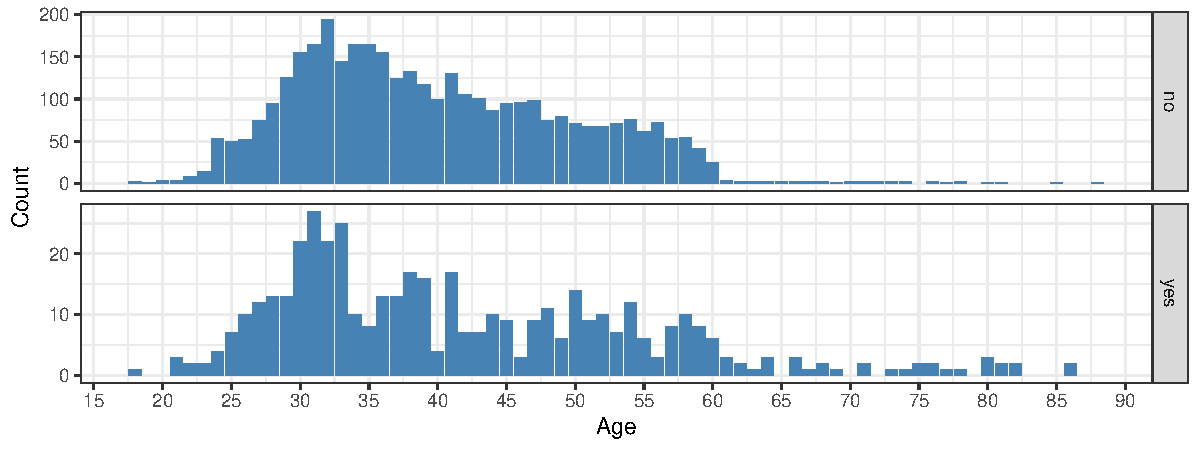
\includegraphics[width=\maxwidth]{figure/unnamed-chunk-17-1} 

}

\caption[New Figure]{New Figure}\label{fig:unnamed-chunk-17}
\end{figure}


\end{knitrout}

\begin{knitrout}
\definecolor{shadecolor}{rgb}{0.969, 0.969, 0.969}\color{fgcolor}\begin{figure}[H]

{\centering 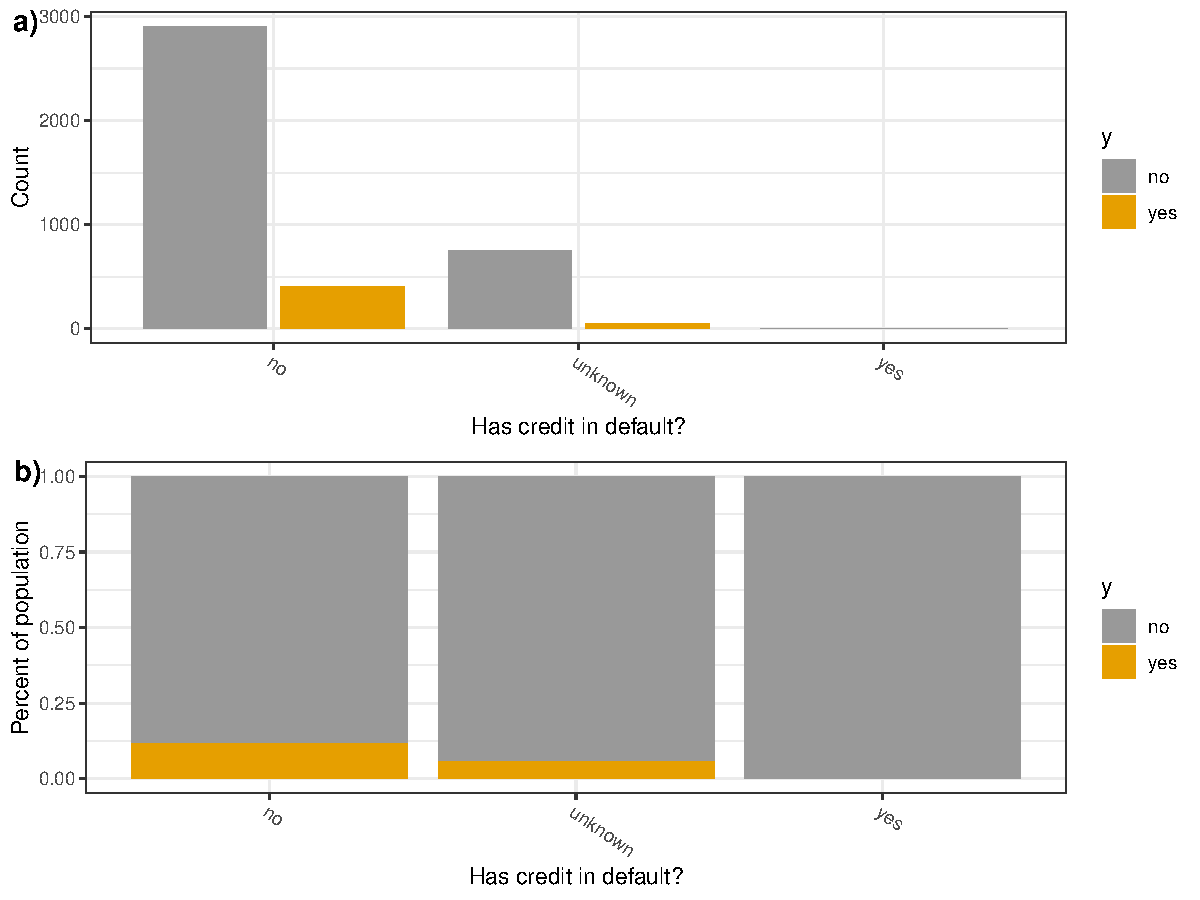
\includegraphics[width=\maxwidth]{figure/unnamed-chunk-18-1} 

}

\caption[New Figure]{New Figure}\label{fig:unnamed-chunk-18}
\end{figure}


\end{knitrout}

\begin{knitrout}
\definecolor{shadecolor}{rgb}{0.969, 0.969, 0.969}\color{fgcolor}\begin{kframe}


{\ttfamily\noindent\bfseries\color{errorcolor}{\#\# Error in dimnames(x) <- dnx: 'dimnames()' zastosowane do nie-tablicy}}\end{kframe}
\end{knitrout}



\subsection{}



\begin{knitrout}
\definecolor{shadecolor}{rgb}{0.969, 0.969, 0.969}\color{fgcolor}\begin{figure}[H]

{\centering 
\includegraphics[width=\maxwidth]{figure/unnamed-chunk-21-1} 

}

\caption[New Figure]{New Figure}\label{fig:unnamed-chunk-21}
\end{figure}


\end{knitrout}

\begin{knitrout}
\definecolor{shadecolor}{rgb}{0.969, 0.969, 0.969}\color{fgcolor}\begin{figure}[H]

{\centering 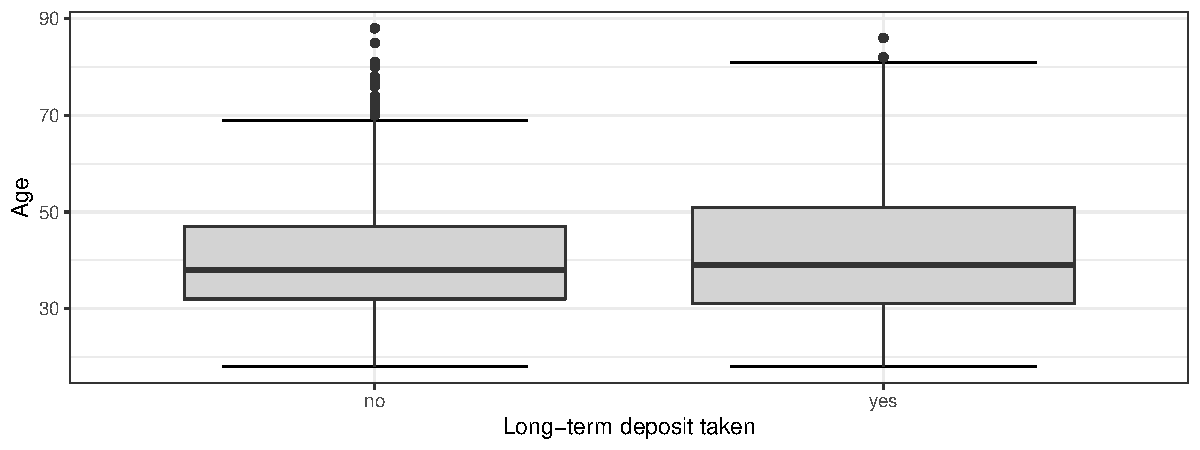
\includegraphics[width=\maxwidth]{figure/unnamed-chunk-22-1} 

}

\caption[New Figure]{New Figure}\label{fig:unnamed-chunk-22}
\end{figure}


\end{knitrout}

\begin{knitrout}
\definecolor{shadecolor}{rgb}{0.969, 0.969, 0.969}\color{fgcolor}\begin{kframe}


{\ttfamily\noindent\bfseries\color{errorcolor}{\#\# Error in dimnames(x) <- dnx: 'dimnames()' zastosowane do nie-tablicy}}\end{kframe}
\end{knitrout}



\subsection{}



\begin{knitrout}
\definecolor{shadecolor}{rgb}{0.969, 0.969, 0.969}\color{fgcolor}\begin{figure}[H]

{\centering 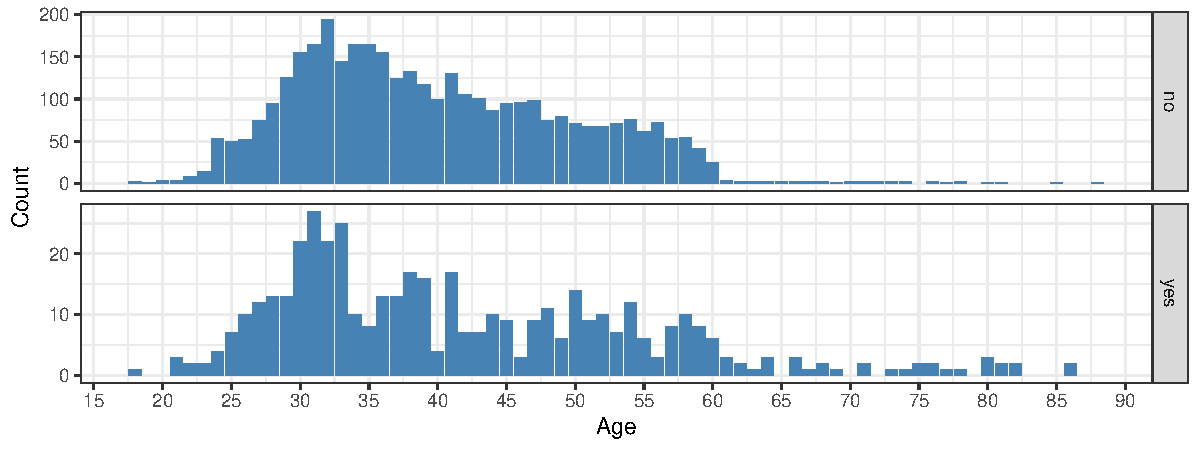
\includegraphics[width=\maxwidth]{figure/unnamed-chunk-25-1} 

}

\caption[New Figure]{New Figure}\label{fig:unnamed-chunk-25}
\end{figure}


\end{knitrout}

\begin{knitrout}
\definecolor{shadecolor}{rgb}{0.969, 0.969, 0.969}\color{fgcolor}\begin{figure}[H]

{\centering 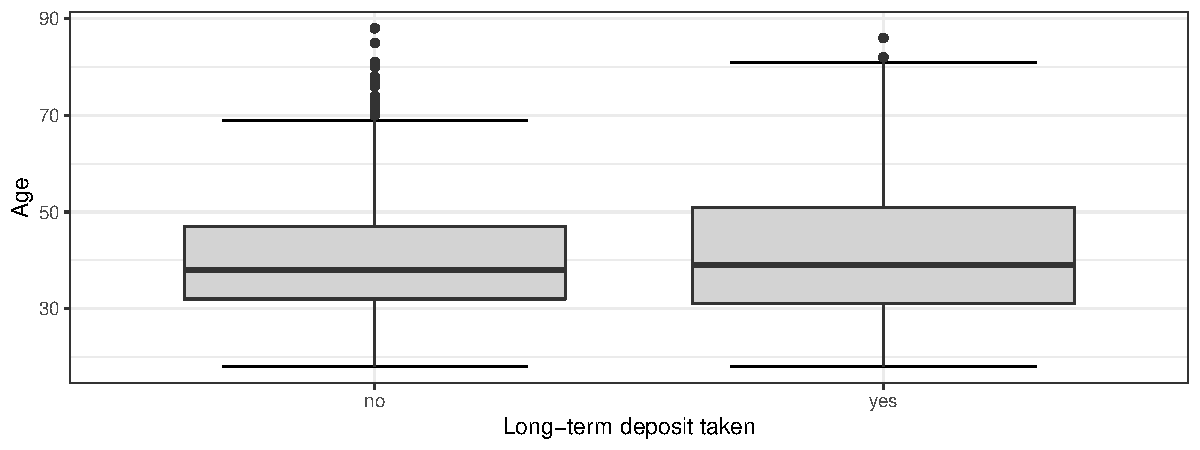
\includegraphics[width=\maxwidth]{figure/unnamed-chunk-26-1} 

}

\caption[New Figure]{New Figure}\label{fig:unnamed-chunk-26}
\end{figure}


\end{knitrout}

\begin{knitrout}
\definecolor{shadecolor}{rgb}{0.969, 0.969, 0.969}\color{fgcolor}\begin{kframe}


{\ttfamily\noindent\bfseries\color{errorcolor}{\#\# Error in dimnames(x) <- dnx: 'dimnames()' zastosowane do nie-tablicy}}\end{kframe}
\end{knitrout}



\subsection{}



\begin{knitrout}
\definecolor{shadecolor}{rgb}{0.969, 0.969, 0.969}\color{fgcolor}\begin{kframe}


{\ttfamily\noindent\bfseries\color{errorcolor}{\#\# Error in dimnames(x) <- dnx: 'dimnames()' zastosowane do nie-tablicy}}\end{kframe}
\end{knitrout}

\begin{knitrout}
\definecolor{shadecolor}{rgb}{0.969, 0.969, 0.969}\color{fgcolor}\begin{figure}[H]

{\centering 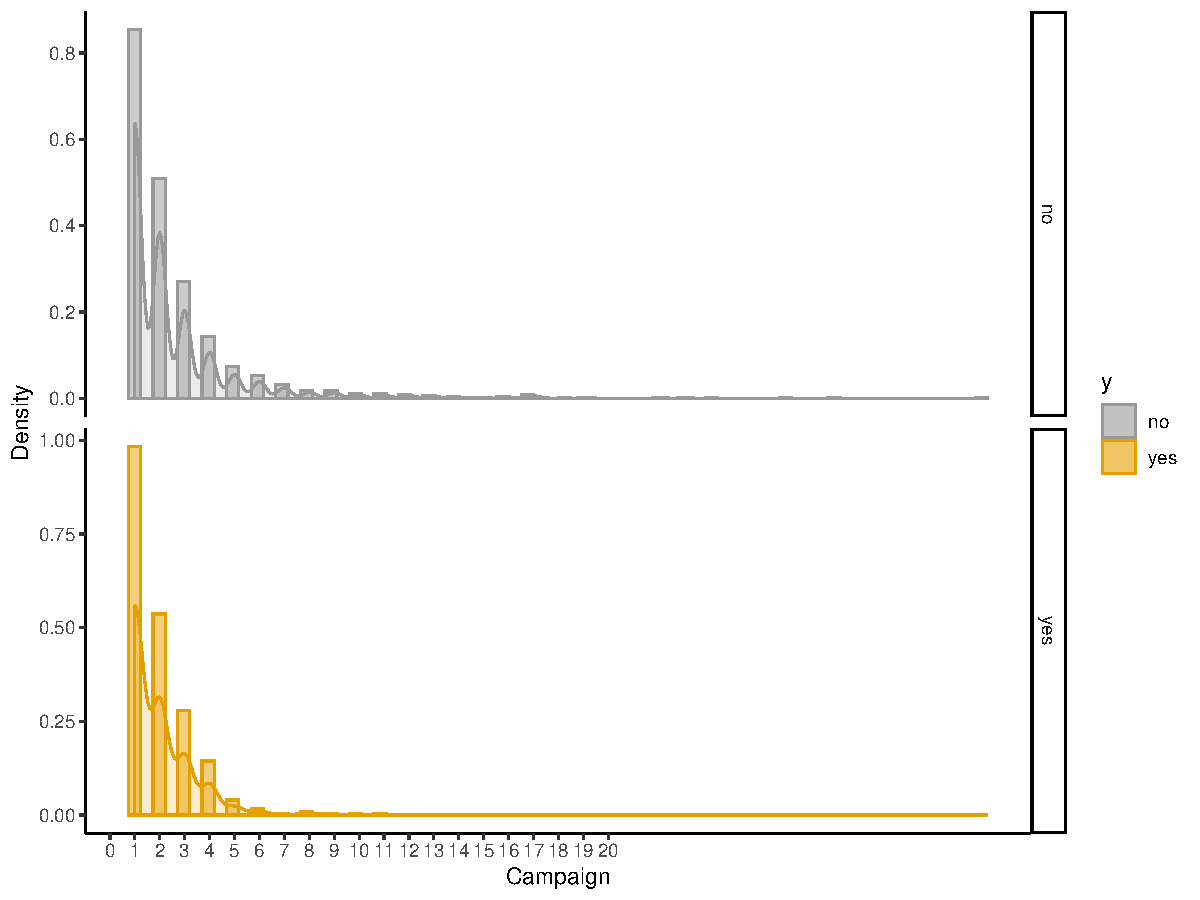
\includegraphics[width=\maxwidth]{figure/unnamed-chunk-30-1} 

}

\caption[New Figure]{New Figure}\label{fig:unnamed-chunk-30}
\end{figure}


\end{knitrout}

\begin{knitrout}
\definecolor{shadecolor}{rgb}{0.969, 0.969, 0.969}\color{fgcolor}\begin{figure}[H]

{\centering 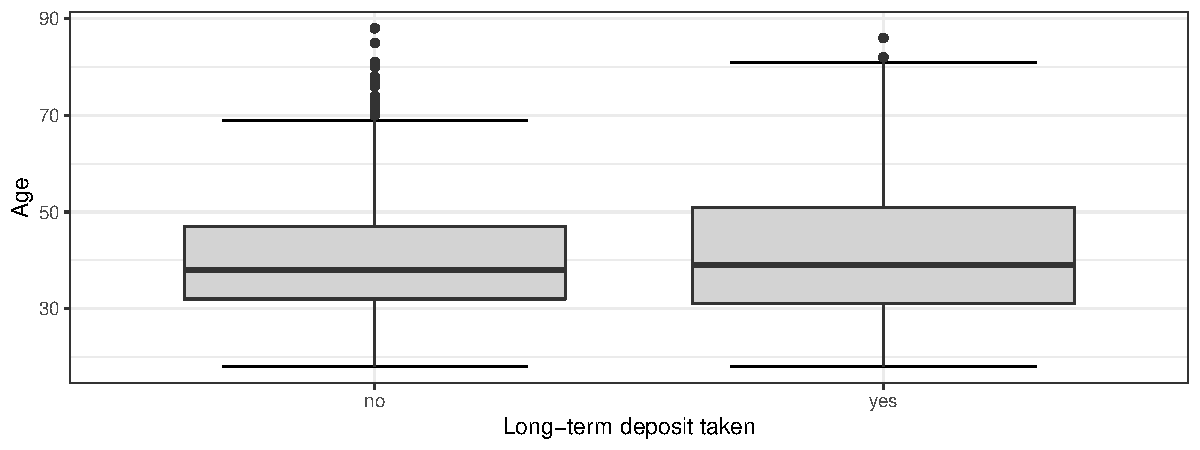
\includegraphics[width=\maxwidth]{figure/unnamed-chunk-31-1} 

}

\caption[New Figure]{New Figure}\label{fig:unnamed-chunk-31}
\end{figure}


\end{knitrout}































\end{document}
